The decision was made to try and adapt the YOLOv4\cite{yolov4} architecture, based on a CSVDarknet53 backbone, to archaeological object detection by applying modifications inspired from the State of the Art object detection methods in satellite imagery detection. Those modifications mostly concerned feature fusion, and receptive field improvements by way of dilated convolution.

\section{Feature Fusion}
Feature Fusion is a technique used in most \glspl{cnn}. The main issue with Deep Networks is that, as the input is convoluted as goes further into the network, the feature maps contains more and more semantic and less geometric information. In other words, deeper feature maps incorporates information as to \textit{what is it} and less about \textit{where is it/what does it looks like}. Moreover, since the feature maps gradually become smaller and smaller, by way of max-pooling, stride of convolution or otherwise, this means that the receptive field or \textit{what the layer is actually sensing} becomes coarser and coarser. Small objects can be missed, since they disappear during the downscaling.

Feature Fusion aims at mitigating this loss by adding information coming from earlier feature maps. Traditional networks usually uses "Skip Connections" to achieve this. ResNet\cite{resNet} simply uses vector addition to add the weight matrices in its Residual Modules. DenseNet\cite{denseNet} concatenates the weight matrices from earlier layer to later ones along the channel dimensions.

\section{Backbone and activation}
The backbone is CSPDarknet53\cite{CSPDarknet53}, most notably used in YOLOv4\cite{yolov4}. This backbone obtained better result than the CSPResNeXt-50\cite{resNeXt} in the \gls{yolo} paper, which is why it is used. Inspiration could also be taken from Zhuang \textit{et al.}\cite{zhuang2019}, with passthrough and concatenation from earlier layers.

\begin{figure}[H]
	\centering
	\includegraphics[width=0.75\textwidth]{darknet53Archi.png}
	\caption[]{Architecture of the Darknet 53 backbone}
	\label{}
\end{figure}

\section{Activation Functions}
The performance of different activation functions will be tested. Mish\cite{mish}(Figure~\ref{fig:mish}) and Swish (Figure~\ref{fig:swish}) or even Scaled Exponential Linear Unit (SELU) (Figure~\ref{fig:selu}) are good candidates. 

\subsection{Scaled Exponential Linear Unit}
\gls{SELU} is one of the first activation developed to address the issue of normalisation in \gls{fnn}: as those networks become deeper and deeper, they become more and more sensitive to gradient issues. Usually, Batch Normalisation is used to mitigate this, but this makes \gls{fnn} sensitive to normalisation during training. \textbf{\glspl{selu} has been developed to incorporate normalisation inside the activation function.}

\gls{selu} is defined by the following equation:
\begin{equation}
	  \sigma[x]=\lambda \begin{cases}
	  	x\\
                \alpha * exp[x] - \lambda 
	  \end{cases}
\end{equation}

With $\alpha$ and $\lambda$ being fixed parameters who are derived from the inputs. In the Figure~\ref{fig:selu}, the values used are for standard scaled inputs with a 0 mean and a 1 standard deviation: $\alpha=1.6732$ and $\lambda=1.0507$. 

\begin{figure}[H]
	\centering
			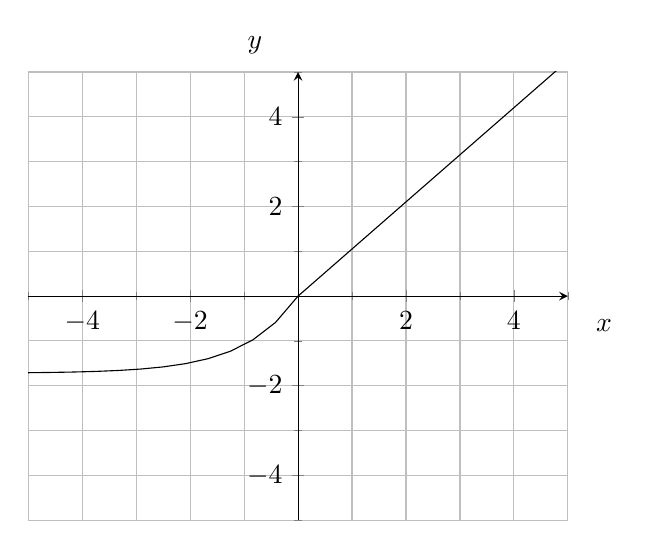
\begin{tikzpicture}
				\begin{axis}[grid=both,ymin=-5,ymax=5,xmax=5,xmin=-5, minor tick num=1,axis lines = middle,xlabel=$x$,ylabel=$y$,label style = {at={(ticklabel cs:1.1)}}]
					\addplot[domain=0:10] {1.0507*x};
					\addplot[domain=-10:0] {1.0507*(1.6372*exp(x) - 1.6372)};
				\end{axis}
			\end{tikzpicture}
		}
		\caption{Scaled Exponential Linear Unit (SELU) Activation Function}
		\label{fig:selu}
\end{figure}



\subsection{Swish}
Swish\cite{swish} is a part of a recent push in research toward a better activation function to replace ReLU. While ReLU offers very good performance, it is not smooth due to the non differentiable point at $x = 0$, and is always zero for all $x < 0$ which can imper learning. Swish has been developped by Google Brain to address those issues, and can be defined as follow:
\begin{equation}
	\sigma[x, \beta] = x \cdot (1 + exp[-\beta x])^{-1}
\end{equation}

Where $(1 + exp[-\beta x])^{-1}$ is the sigmoid function and where $\beta$ is either a constant or a training \gls{hyperparameter}. If $\beta = 1$, then Swish is equivalent to the weighed Sigmoid-Weighted Linear Unit (SiL). If $\beta = 0$, then Swish becomes the scaled linear function $f[x] = 0.5 \cdot x$. As $\beta \leftarrow \infty$, Swish approaches a $0-1$ function, like the ReLU. In other words, Swish can be interpreted as \textbf{a non linear interpolation between the linear function and the ReLU function, which degree of interpolation can be controlled by the model if $\beta$ is set as a trainable parameter}
	\begin{figure}[H]
		\centering
			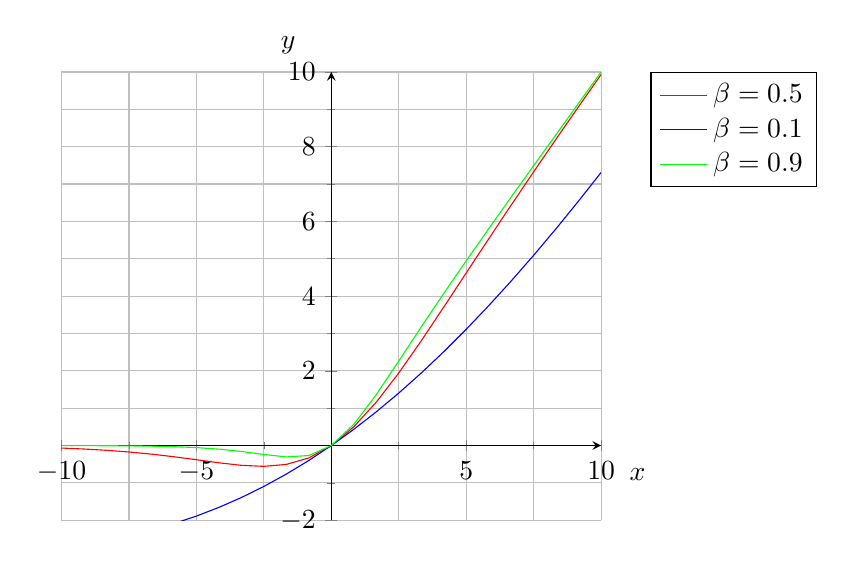
\begin{tikzpicture}[]
				\begin{axis}[grid=both,ymin=-2,ymax=10,xmax=10,xmin=-10, minor tick num=1,axis lines = middle,xlabel=$x$,ylabel=$y$,label style = {at={(ticklabel cs:1.1)}}, legend style={at={(1.4, 1)},anchor=north east}]
					\addplot[red, domain=-10:10] {x*1/(exp(-0.5*x)+1)};
					\addlegendentry{$\beta = 0.5$}
					\addplot[blue, domain=-10:10] {x*1/(exp(-0.1*x)+1)};
					\addlegendentry{$\beta = 0.1$}
					\addplot[green, domain=-10:10] {x*1/(exp(-0.9*x)+1)};
					\addlegendentry{$\beta = 0.9$}
				\end{axis}
			\end{tikzpicture}
		
			\caption{The Swish activation function, with different values of $\beta$}
			  \label{fig:swish}
	\end{figure}

\subsection{Mish}
Mish is a novel activation function which has been proposed by Misra\cite{mish} to act as a replacement for the immensely popular ReLU function.  Mish is built as a successor for ReLU and is inspired by the Swish function, described above. Mish is very simple, and defined as below: 
\begin{equation}
	\sigma[x] = x \cdot \text{tanh}[1 + exp[x]]
\end{equation}

Similar to Swish, Mish is unbounded above, preventing saturation, but bounded below, creating a self-regularisation. Mish has an order of continuity $C^\infty$, a preferable property over ReLU having a $C^0$, which can cause problem in gradient-based optimisation. Finally, Mish is non monotonic, which causes small negative inputs to be preserved as negative outputs. Mish obtains improve performance by up to 1.6\% on dataset such as the MNIST\cite{mnist} or CIFAR-10\cite{cifar}

\begin{figure}[h]
	\centering
	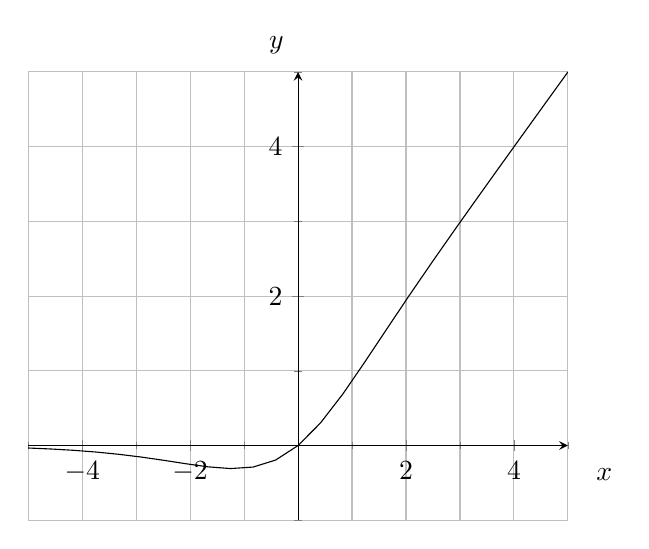
\begin{tikzpicture}[]
				\begin{axis}[grid=both,ymin=-1,ymax=5,xmax=5,xmin=-5, minor tick num=1,axis lines = middle,xlabel=$x$,ylabel=$y$,label style = {at={(ticklabel cs:1.1)}}]
					\addplot[] {x*tanh(ln(1+exp(x))};
				\end{axis}

	\end{tikzpicture}
	\caption{The mish activation function}
	\label{fig:mish}
\end{figure}


\section{Dual Scale Detectors}
An idea introduced in YOLT\cite{yolt} is to use two different detectors running simultaneously: one trained on small scale images to detect small objects, the other trained on larger images to detect bigger objects. The small scale network would be fed small chips of images, while the large scale network would be fed downscaled large swathes of terrain. This meant that the large scale network would run much less often than the small scale network, and mitigate the loss of performance of running two network at the same time.

An ensemble method similar to this could be used, where two networks try to find objects at different scales.

\section{Multi-scale Feature Fusion}
To be able to detect the small objects often seen in \gls{lidar} data, some kind of \gls{mlff} module needs to be used. There are a few existing modules and techniques that can boost the detection rates of a model by aggregating low level feature maps from earlier layers with ones from higher layers.  

The \gls{mlff} module from Zhuang \textit{et al.}\cite{zhuang2019} takes 3 feature maps from different layers, upscales and concatenates them, then applies a series of convolution operations to obtain 3 predictions at different scale. This is very similar to the \gls{mlff} used in YOLOv3\cite{yolov3}, where 3 predictions are made at different scale level and which reuses feature maps from deeper layers to build the predictions.

\begin{figure}[H]
	\centering
	\includegraphics[width=\textwidth]{msFusionDetectorArchi}
	\caption[Feature Fusion in Zhuang \textit{et al.}]{Feature Fusion implementation of Zhuang \textit{et al.}. We are only interested in the bottom part of the figure, with feature maps from different levels being concatenated.}
	\label{fig:mlffZhuang}
\end{figure}

The \gls{mlff} module from Qian \textit{et al.}\cite{qianAl} shown in Figure~\ref{fig:mlffQian} takes each proposal generated by a \gls{rpn}, and maps its position to all level of feature map generated by the \gls{fpn}. From there it obtains $N$ regions of the feature maps ($N$ being the number of levels), which it transforms into $7 \times 7$ feature maps through the RoiAlign\cite{maskrcnn} operation. Finally, it concatenates these 4 regions along the channel dimensions, and applies two convolution operations along with a Fully Connected Layer for bounding box regression and classification.

\begin{figure}[H]
	\centering
	\includegraphics[width=\textwidth]{ODRSIArchi}
	\caption[Architecture of Qian \textit{et al.}]{Architecture of the model from Qian et al. We are interested in the module shown in (b), where particular regions of different feature maps are concatenated together}
	\label{fig:mlffQian}
\end{figure}

The \gls{pan} is a sort of multi layer feature fusion module. Following the same principle as the \gls{mlff} from Qian \textit{et al.}, \gls{pan} takes the features maps generated by a \gls{fpn}. It first downscales the lower level layer (denoted $P_i$ with a $3 \times 3$ convolution operation with a stride of 2. It then adds element wise this downscaled layer with the layer $P_{i+1}$. This is done iteratively until the up most layer is attained. \textbf{In the YOLOv4 paper, instead of adding the layers, a concatenation is done}.

\begin{figure}[H]
	\centering
	\begin{subfigure}[b]{0.3\textwidth}
		\centering
		\includegraphics[width=\textwidth]{pan}
		\caption{PAN}
		\label{fig:pan}
	\end{subfigure}
	\begin{subfigure}[b]{0.3\textwidth}
		\centering
		\includegraphics[width=\textwidth]{panMod}
		\caption{Modified PAN}
		\label{fig:panmod}
	\end{subfigure}
	\caption{PAN and its YOLO modification}
	\label{fig:PAN}
\end{figure}

\section{Receptive Field Improvements}

To improve the size of the receptive field, the modified \gls{spp} module from YOLOv3\cite{yolov3} would be used. Experimentations could be done using dilated convolutions, as seen in Yu \textit{et al.}\cite{yu2015} and Ju \textit{et al.}. Dilated convolution improve the receptive field by increasing the kernel size without increasing the number of parameters in the kernel. This can help reducing the number of parameters, improving performance of the network in terms of \gls{fps}. We can replace some of the classical convolution blocks from the CSPDarknet53 backbone with dilated convolution modules, as can be seen in Figure~\ref{fig:dilConvDarknet}. 

\begin{figure}[H]
	\centering
	\includegraphics[width=\textwidth]{archiDilConv}
	\caption[]{General Architecture of the Darknet Backbone with a dilated convolution module replacing a convolution block}
	\label{fig:dilConvDarknet}
\end{figure}

\section{Attention Modules}
Attention modules are used to improve the accuracy of detections network by increasing the importance of particular regions or channels. The \gls{sam}\cite{sam} would be used, as it increases the accuracy without significantly impacting inference speed. Testing would have to be done to evaluate whether the \gls{sam} improvement done by Bochkovsky \textit{et al.} in the YOLOv4 paper\cite{yolov4} gives out a performance increase.

\begin{figure}[H]
	\centering
	\begin{subfigure}[b]{0.4\textwidth}
		\centering
		\includegraphics[width=\textwidth]{sam}
		\caption{\gls{sam}}
		\label{fig:samnorm}
	\end{subfigure}
	\begin{subfigure}[b]{0.4\textwidth}
		\centering
		\includegraphics[width=\textwidth]{samMod}
		\caption{Modified \gls{sam}}
		\label{fig:samod}
	\end{subfigure}
	\caption{SAM and its YOLO modification}
	\label{fig:SAM}
\end{figure}

\section{Post-processing}
\gls{nms} needs to be used to remove the superfluous bounding boxes generated by the network. Soft Non maximum suppression, as introduced by Qian \textit{et al.} \cite{qianAl} would be used to achieve such a task, while trying to not miss the smaller objects.


\section{List of all the possible testing arrangements}
We will need to test a multiple of different modifications on the base CSPDarknet-53 and test out if those modifications results in performances improvements.
\begin{itemize}
	\item Double YOLOv4 trained on large and small scale (similar to YOLT\cite{yolt})
	\item CSPDarknet with one or two dilated convolution modules
	\item \gls{mlff} module from Zhuang \textit{et al.}: see Figure~\ref{fig:mlffZhuang}
	\item \gls{mlff} module from Qian \textit{et al.}: see Figure~\ref{fig:mlffQian}
	\item Modified PAN module: see Figure~\ref{fig:PAN}
	\item Modified SAM Module: see Figure~\ref{fig:SAM}
	\item Different activations: ReLU, Leaky ReLU, \gls{selu}, Mish or Swish
	\item Different activations: Different \glspl{iou}: \gls{giou}, \gls{ciou}, \gls{diou} 
	\item Various input resolutions 
\end{itemize}


Now State of the Art methods uses more dedicated techniques to fuses information from different depths. Usually multiple predictions are done at different depths levels, and incorporates information from all layers.  YOLOv3\cite{yolov3} also uses multi-scale predictions to improve performance. \textbf{Leveraging the power of those techniques is key in enhancing the performance on deep learning models in high resolution - small scale object detection.}

\section{YOLOv4}
The latest version of the \gls{yolo} architecture is used as a base to modify. \gls{yolo} is a state of the art detector, obtaining extremely good results on a variety of datasets, and with the benefits of still being extremely fast: it is capable of running on real time will requiring only a modest amount of processing power. YOLOv4 is the latest iteration of this architecture, incorporating the latest and best modifications and improvement on the always growing class of object detectors. For a review on those improvements, please refer to section~\ref{yolov4}. 

